\chapter{ Технологический раздел}
\label{cha:technological}

    В данном разделе будут выбраны средства реплизации ПО, представлен листинг кода
    и проведён теоритический анализ максимальной затрачиваемой памяти. 

    \section{Средства реализации}
        В данной работе используется язык программирования python \cite{python}, так как
        он позволяет написать программу в относительно малый срок.
        В качестве среды разработки использовалась Visual Studio Code \cite{visual-studio-code}.

        Для замера процессорного времени была использована функция process\_time \cite{process_time} модуля time.
        Она возвращает значение в долях секунды суммы системного и пользовательского процессорного времени текущего процесса и 
        не включает время, прошедшее во время сна.

    \section{Листинг программы}
        Ниже представлены листинги кода умножения матриц:
        \begin{enumerate}
            \item стандартной реализации (листинг \ref{lst:standartDot});
            \item реализация алгоритма Винограда (листинг \ref{lst:vinogradDot});
            \item реализация оптимизированного алгоритма Винограда (листинг \ref{lst:vinogradDot:optimize}).
        \end{enumerate}
        
        \begin{lstlisting}[language=python, label=lst:standartDot, caption=Реализация классического алгоритма умножения матриц]
def dotMatrix(matr_a : list, matr_b: list) -> (list, float):
    if (len(matr_b) != len(matr_a[0])):
        raise ValueError
    
    m = len(matr_a)
    n = len(matr_a[0])
    q = len(matr_b[0])
    matr_c = [[0] * q for i in range(m)]

    t_start = process_time()
    for i in range(m):
        for j in range(q):
            for k in range(n):
                matr_c[i][j] = matr_c[i][j] + matr_a[i][k] * matr_b[k][j]
    t_end = process_time()

    return matr_c, t_end - t_start
        \end{lstlisting}

        \begin{lstlisting}[language=python, label=lst:vinogradDot, caption=Реализация алгоритма Винограда умножения матриц]
def dotMatrixVinograd(matr_a : list, matr_b: list) -> (list, float):
    if (len(matr_b) != len(matr_a[0])):
        raise ValueError
    
    m = len(matr_a)
    n = len(matr_a[0])

    q = len(matr_b[0])
    matr_c = [[0] * q for i in range(m)]

    row = [0] * m
    col = [0] * q

    t_start = process_time()

    for i in range(m):
        for j in range(n // 2):
            row[i] = row[i] + matr_a[i][2*j] * matr_a[i][2*j + 1]
    
    for j in range(q):
        for i in range(n // 2):
            col[j] = col[j] + matr_b[2*i][j] * matr_b[2*i+1][j]

    for i in range(m):
        for j in range(q):
            matr_c[i][j] = -row[i] - col[j]
            for k in range(n//2):
                matr_c[i][j] = matr_c[i][j] + (matr_a[i][2*k+1] + matr_b[2*k][j]) * (matr_a[i][2*k] + matr_b[2*k+1][j])

    if n % 2:
        for i in range(m):
            for j in range(q):
                matr_c[i][j] = matr_c[i][j] + matr_a[i][n-1] * matr_b[n-1][j]
    t_end = process_time()

    return matr_c, t_end - t_start
        \end{lstlisting}

        \begin{lstlisting}[language=python, label=lst:vinogradDot:optimize, caption=Реализация оптимизированного алгоритма Винограда умножения матриц]
def dotMatrixVinogradOptimizate(matr_a : list, matr_b: list) -> (list, float):
    if (len(matr_b) != len(matr_a[0])):
        raise ValueError
    
    m = len(matr_a)
    n = len(matr_a[0])
    q = len(matr_b[0])
    matr_c = [[0] * q for i in range(m)]

    row = [0] * m
    col = [0] * q
    t_start = process_time()
    for i in range(m):
        for j in range(1, n, 2):
            row[i] -= matr_a[i][j] * matr_a[i][j - 1]
    
    for j in range(q):
        for i in range(1, n, 2):
            col[j] -= matr_b[i][j] * matr_b[i - 1][j]

    for i in range(m):
        for j in range(q):
            matr_c[i][j] = row[i] + col[j]
            for k in range(1, n, 2):
                matr_c[i][j] += (matr_a[i][k - 1] + matr_b[k][j]) * (matr_a[i][k] + matr_b[k-1][j])

    if n % 2:
        for i in range(m):
            for j in range(q):
                matr_c[i][j] += matr_a[i][n-1] * matr_b[n-1][j]
    t_end = process_time()

    return matr_c, t_end - t_start
        \end{lstlisting}
    
        
    \section{Тестирование}
        В таблице \ref{table:testing} отображён возможный набор тестов
        для тестирования методом чёрного ящика, результаты которого, 
        представленные на рисунке \ref{png:testing:result}, подтверждают
        прохождение программы перечисленных тестов.

        \begin{table}[]
            \caption{Тесты для проверки корректности программы}

            \centering
            \begin{tabular}{|c|c|c|}
                \hline
                Матрица A                                                & Матрица B                                              & Ожидаемый результат                                    \\ \hline
                $\begin{bmatrix} 0 & 0 \\ 0 & 0 \end{bmatrix}$           & $\begin{bmatrix} 1 & 1 & 1 \\ 1 & 1 & 1 \end{bmatrix}$ & $\begin{bmatrix} 0 & 0 & 0 \\ 0 & 0 & 0 \end{bmatrix}$ \\ \hline
                $\begin{bmatrix} 1 & 0 \\ 0 & 1 \end{bmatrix}$           & $\begin{bmatrix} 1 & 1 & 1 \\ 1 & 1 & 1 \end{bmatrix}$ & $\begin{bmatrix} 1 & 1 & 1 \\ 1 & 1 & 1 \end{bmatrix}$ \\ \hline
                $\begin{bmatrix} 1 & 1 \\ 1 & 1 \\ 1 & 1 \end{bmatrix}$  & $\begin{bmatrix} 1 & 1 & 1 \\ 1 & 1 & 1 \end{bmatrix}$ & $\begin{bmatrix} 2 & 2 & 2 \\ 2 & 2 & 2 \\ 2 & 2 & 2 \end{bmatrix}$ \\ \hline
                $\begin{bmatrix} 1 \\ 1 \end{bmatrix}$                   & $\begin{bmatrix} 1 & 1 & 1 \\ 1 & 1 & 1 \end{bmatrix}$ & the matrices cannot be multiplied                       \\ \hline
                \end{tabular}
            \label{table:testing}
        \end{table}
        
        \begin{figure}[h!]
            \centering
            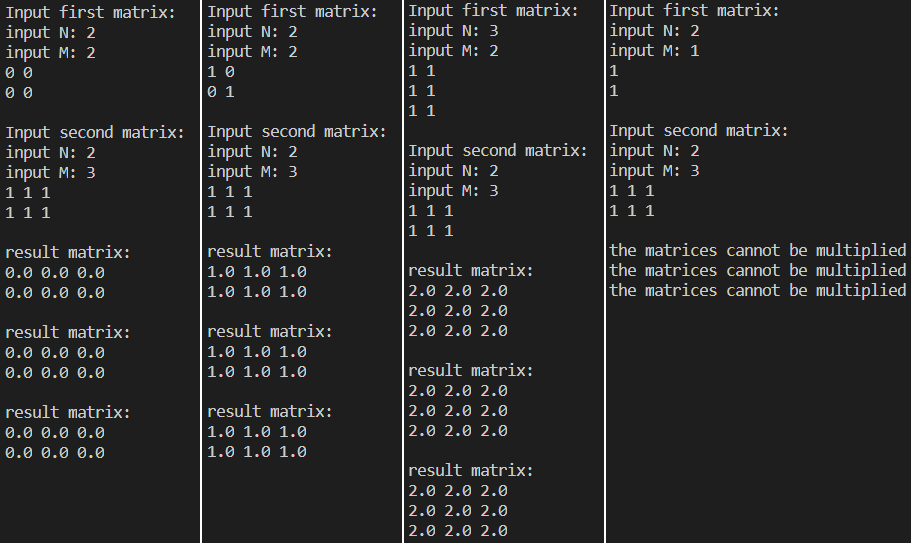
\includegraphics[scale=0.9]{testing.png}
            \caption{Результаты тестирования алгоритмов: стандартного, Винограда и оптимизированного Винограда}
            \label{png:testing:result}
        \end{figure}
\newpage